\section{Theorie}
\section{Theorie}
\label{sec:Theorie}


\subsection{Zielsetzung}
Bei diesem Versuch sollen Störstellen in einem Acrylblock mithilfe eines A-Scans und
mit einem B-Scan untersucht und vermessen werden, zudem soll die Auflösung verschiedener
Sonden verglichen werden.
Außerdem soll mit einem TM-Scan die Frequenz und das Herzvolumen eines Herzmodells untersucht werden.


\subsection{Theorie}
Ultraschall liegt in einem Frequenzbereich von etwa 20\;kHz bis 1\;GHz, sodass diese
Schallwellen vom menschlichen Gehör nicht erfasst werden können. Überschreiten Schallwellen den
Frequenzbereich von Ultraschall, sodass sie über 1\;GHz liegen, werden diese als Hyperschall bezeichnet.
Genutzt wird Ultraschall häufig in der Medizin für biometrische Messungen, sowie in
der zerstörungsfreien Werkstoffprüfung.

Schallwellen breiten sich durch Druckschwankungen fort und beschreiben eine
longitudinale Welle mit
\begin{equation}
  p(x,t)= p_0 +v_0 Z\cos{(\omega t - k x)}.
  \label{longitud}
\end{equation}

Dabei wird die akustische Impedanz (oder Schallkennwiderstand) als $Z=c\cdot\rho$
definiert, wobei $c$ die Schallgeschwindigkeit im Material beschreibt und $\rho$
die Dichte.
Schallwellen besitzen viele Ähnlichkeiten zu elektromagnetischen Wellen,
beispielsweise können das Reflexions- und Brechungsverhalten analog beschrieben werden. \\
Allerdings ist die Ausbreitungsgeschwindigkeit deutlich geringer und hängt zudem
stark vom Medium ab. In einer Flüssigkeit hängt die Schallgeschwindigkeit insbesondere von der Dichte $\rho$ und der Kompressibilität $\kappa$
gemäß
\begin{equation}
  c_{FL}=\sqrt{\frac{1}{\kappa \rho}}.
  \label{cfl}
\end{equation}
ab. In Gasen und Flüssigkeiten breitet sich Schall immer als Longitudinalwelle aus,
jedoch können sich in Festkörpern aufgrund von Schubspannungen zudem auch
transversale Wellen ausbilden. Hierbei ist die Schallgeschwindigkeit durch die Gleichung
\begin{equation}
  c_{FE}=\sqrt{\frac{E}{\rho}}.
  \label{cfest}
\end{equation}
gegeben, wobei $E$ das Elastizitätsmodul bezeichnet. Jedoch ist die Ausbreitungsgeschwindigkeitin Festkörpern
grundsätzlich richtungsabhängig, insbesondere unterscheiden sich longitudinale und transversale Geschwindigkeit.
\\
Desweiteren kommt es bei der Ausbreitung von Schall auch zu dem Effekt der Absorption, wobei
die  Intensität einer Schallwelle exponentiell mit der Strecke abnimmt, was mit einem Energieverlusst
der Welle verknüpft ist. Diese Abnahme wird durch die Formel
\begin{equation}
  I(x)=I_0\cdot \exp{(-\alpha x)}.
  \label{eqn:intensität}
\end{equation}
beschrieben, hierbei ist $\alpha$ der sogenannte Absorptionskoeffizient.
Luft besitzt einen hohen Absorptionskoeffizienten $\alpha$, da sie Ultraschall in hohem
Maße absorbiert.
Daher wird zwischen der Ultraschallquelle und der Probe meist ein Kontaktmittel verwendet, beispielsweise
destilliertes Wasser oder ein spezielles Kontaktgel.

Trifft eine Schallwelle auf eine Übergang zweier unterschiedlicher Medien, so wird ein Teil der
Welle reflektiert, wobei der
Reflexionskoeffizient $R$ sich mit Hilfe der akustischen Impedanz $Z$
der beiden angrenzenden Materialien durch
\begin{equation}
  R=\Bigl(\frac{Z_1 -Z_2}{Z_1 +Z_2}\Bigr)^{2}.
  \label{refexion}
\end{equation}
berechnen lässt.
Der transmittierte Anteil $T$ lässt sich hingegen durch $T=1-R$ berechenen.


\subsection{Piezo-elektrischer Effekt}
Eine häufig verwendete Methode zur Erzeugung von Ultraschallwellen ist der reziproke piezo-elektrische Effekt,
bei welchem ein piezoelektrischer Kristall in einem elektrischen
Wechselfeld zu Schwingungen angeregt wird. Falls eine polare Achse des Kristalls in
Richtung des elektrischen Feldes zeigt, kommt es zur Emission von Ultraschallwellen,
wobei besonders hohe Schallamplituden und Schallenergiedichten durch Resonanzeffekte
zwischen Anregungsfrequenz und Eigenfrequenz der Kristalle erreicht werden.
\\
Piezokristalle werden zudem zur Detektierung von Ultraschallwellen eingesetzt,
da die eintreffenden Wellen den Kristall zu messbaren Schwingungen anregen.
Obwohl Quarze nur einen schwachen piezoelektrischen Effekt aufweisen, werden sie
am häufigstens als Piezokristalle eingesetzt, da sie über gleichbleibende
physikalische Eigenschaften verfügen.

\subsection{Laufzeitmessungen}

Bei der Laufzeitmessungen werden grundsätzlich zwei Verfahren unterschieden, das Durchschallungsverfahren
und das Impuls-Echo-Verfahren.
Für das Durchschallungsverfahren wird sowohl ein Ultraschallsender als auch ein Ultraschallempfänger benötigt, wie
in Abbildung \ref{fig:durch} dargestellt ist.

\begin{figure}[H]
  \centering
  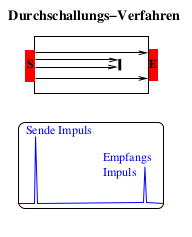
\includegraphics[height=6cm]{durch.png}
  \caption{Schematische Darstellung des Durchschallungsverfahrens.}
  \label{fig:durch}
  \cite{skript}
\end{figure}

Hierbei wird zunächst ein kurzzeitiger Schallimpuls ausgesendet, welcher am anderen Ende
der Probe durch den Empfänger detektiert wird. Falls sich Fehler oder Unebenheiten
in der Probe befinden, wird nur eine abgeschwächte Intensität am
Empfänger gemessen, jedoch ist über die Lage der Fehlerstelle keine genaue Aussage möglich.


Das zweite Verfahren, welches als Impuls-Echo-Verfahren bezeichnet wird,
basiert auf der Nutzung einer einzelnen Sonde als Sender und Empfänger gleichzeitig. Dies ist
schematisch in Abbildung \ref{fig:echo}
dargestellt.

\begin{figure}[H]
  \centering
  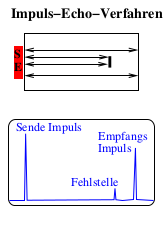
\includegraphics[height=6cm]{echo.png}
  \caption{Schematische Darstellung des  Impuls-Echo-Verfahrens.}
  \label{fig:echo}
  \cite{skript}
\end{figure}

Hierbei wird der ausgesendete Impuls wird am Übergang zweier Medien teilweise reflektiert und nach
dem Rücklaufen durch die Probe vom Empfänger registriert. Ist die Schallgeschwindigkeit
konstant kann über die Laufzeit $t$ die Lage der Fehlstelle über
\begin{equation}
  s=\frac{1}{2}ct
  \label{strecke}
\end{equation}
bestimmt werden.
Im Falle von Fehlstellen, lassen sich durch die Höhe und die Lage der rücklaufenden Impulse
weitere Informationen über die Größe bzw. Beschaffenheit der Fehlstelle gewinnen. \\
Es kann zudem auch zwischen verschiedenen Darstellungsarten dieser Laufzeitmessung
gewählt werden.
Die erste ist der sogenannte A-Scan (Amplituden Scan), bei welchem die Amplituden der rücklaufenden
Echos in Abhängigkeit der Laufzeit dargestellt werden. Dieses Verfahren liefert nur ein
eindimensionales Bild und wird daher meist zur Untersuchung von Strukturen verwendet.\\
Zudem gibt es auch noch den B-Scan (Brightness Scan), bei welchem ein zweidimensionales Bild mittels
Helligkeitsabstufungen des Echos erstellt wird. Außerdem gibt es noch den Time-Motion Scan,
abgekürtzt durch TM-Scan, bei welchem auch die zeiltliche Abfolge von Impulsen augezeichnet
werden kann. Dafür ist eine schnelle Abtastung notwendig; nützlich ist diese Darstellungsart
beispielsweise bei der Untersuchung von Organen.


\subsection{Vorbereitung}
Zur Vorbereitung auf den Versuch wurden materialspeziefische Werte recherchiert, diese
sind in Tabelle \ref{tab:tab1} abzulesen.

\begin{table}[H]
  \centering
  \caption{Werte für die Schallgeschwindigkeit.}
  \label{tab:tab1}
    \begin{tabular}{c |c c c}
    \toprule
    & Luft & dest. Wsser& Acryl\\
    \midrule
    Schallgeschwindigkeit c in m/s & 330 & 1480 & 2730\\
    \bottomrule
    \end{tabular}
    \cite{olympus}, \cite{halle}
  \end{table}

